\chapter{Results}
In this chapter, the results of the project will be discussed. This chapter will be split up into System Integration, Drone Control, Spectrum Sensing, Spectrum Localization, and GPS sections.

\section{System Integration}
This section details the physical system and the integration of the hardware. This includes power consumption, system layout, and component failures or difficulties. The system diagram shown in Figure \ref{fig:masdr_system_diagram} will be explained in detail in this section.
\begin{figure}[ht!]
	\centering
	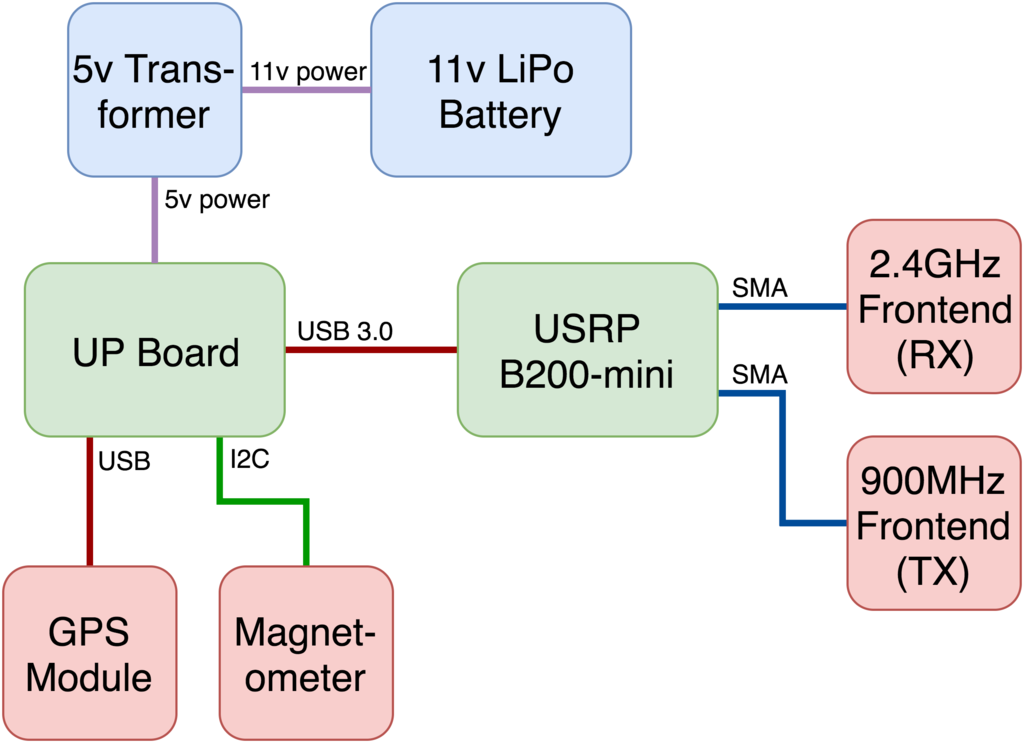
\includegraphics[width=0.70\textwidth]{img/masdr_system_diagram.png}
	\caption{MASDR system diagram detailing the connections between each component.}
	\label{fig:masdr_system_diagram}
\end{figure}\par
The encasing for the system was designed in SOLIDWORKS. It was fabricated using wood panels and a laser cutter. The encasing was designed to be as minimal as possible to reduce the weight of the system. This was done by cutting holes in the panels to remove as much material as possible and using metal supports instead of wooden walls. The metal supports were used in each of the corners to connect the two wooden panels as seen in Figure \ref{fig:connectors}.
\begin{figure}[ht!]
	\centering
	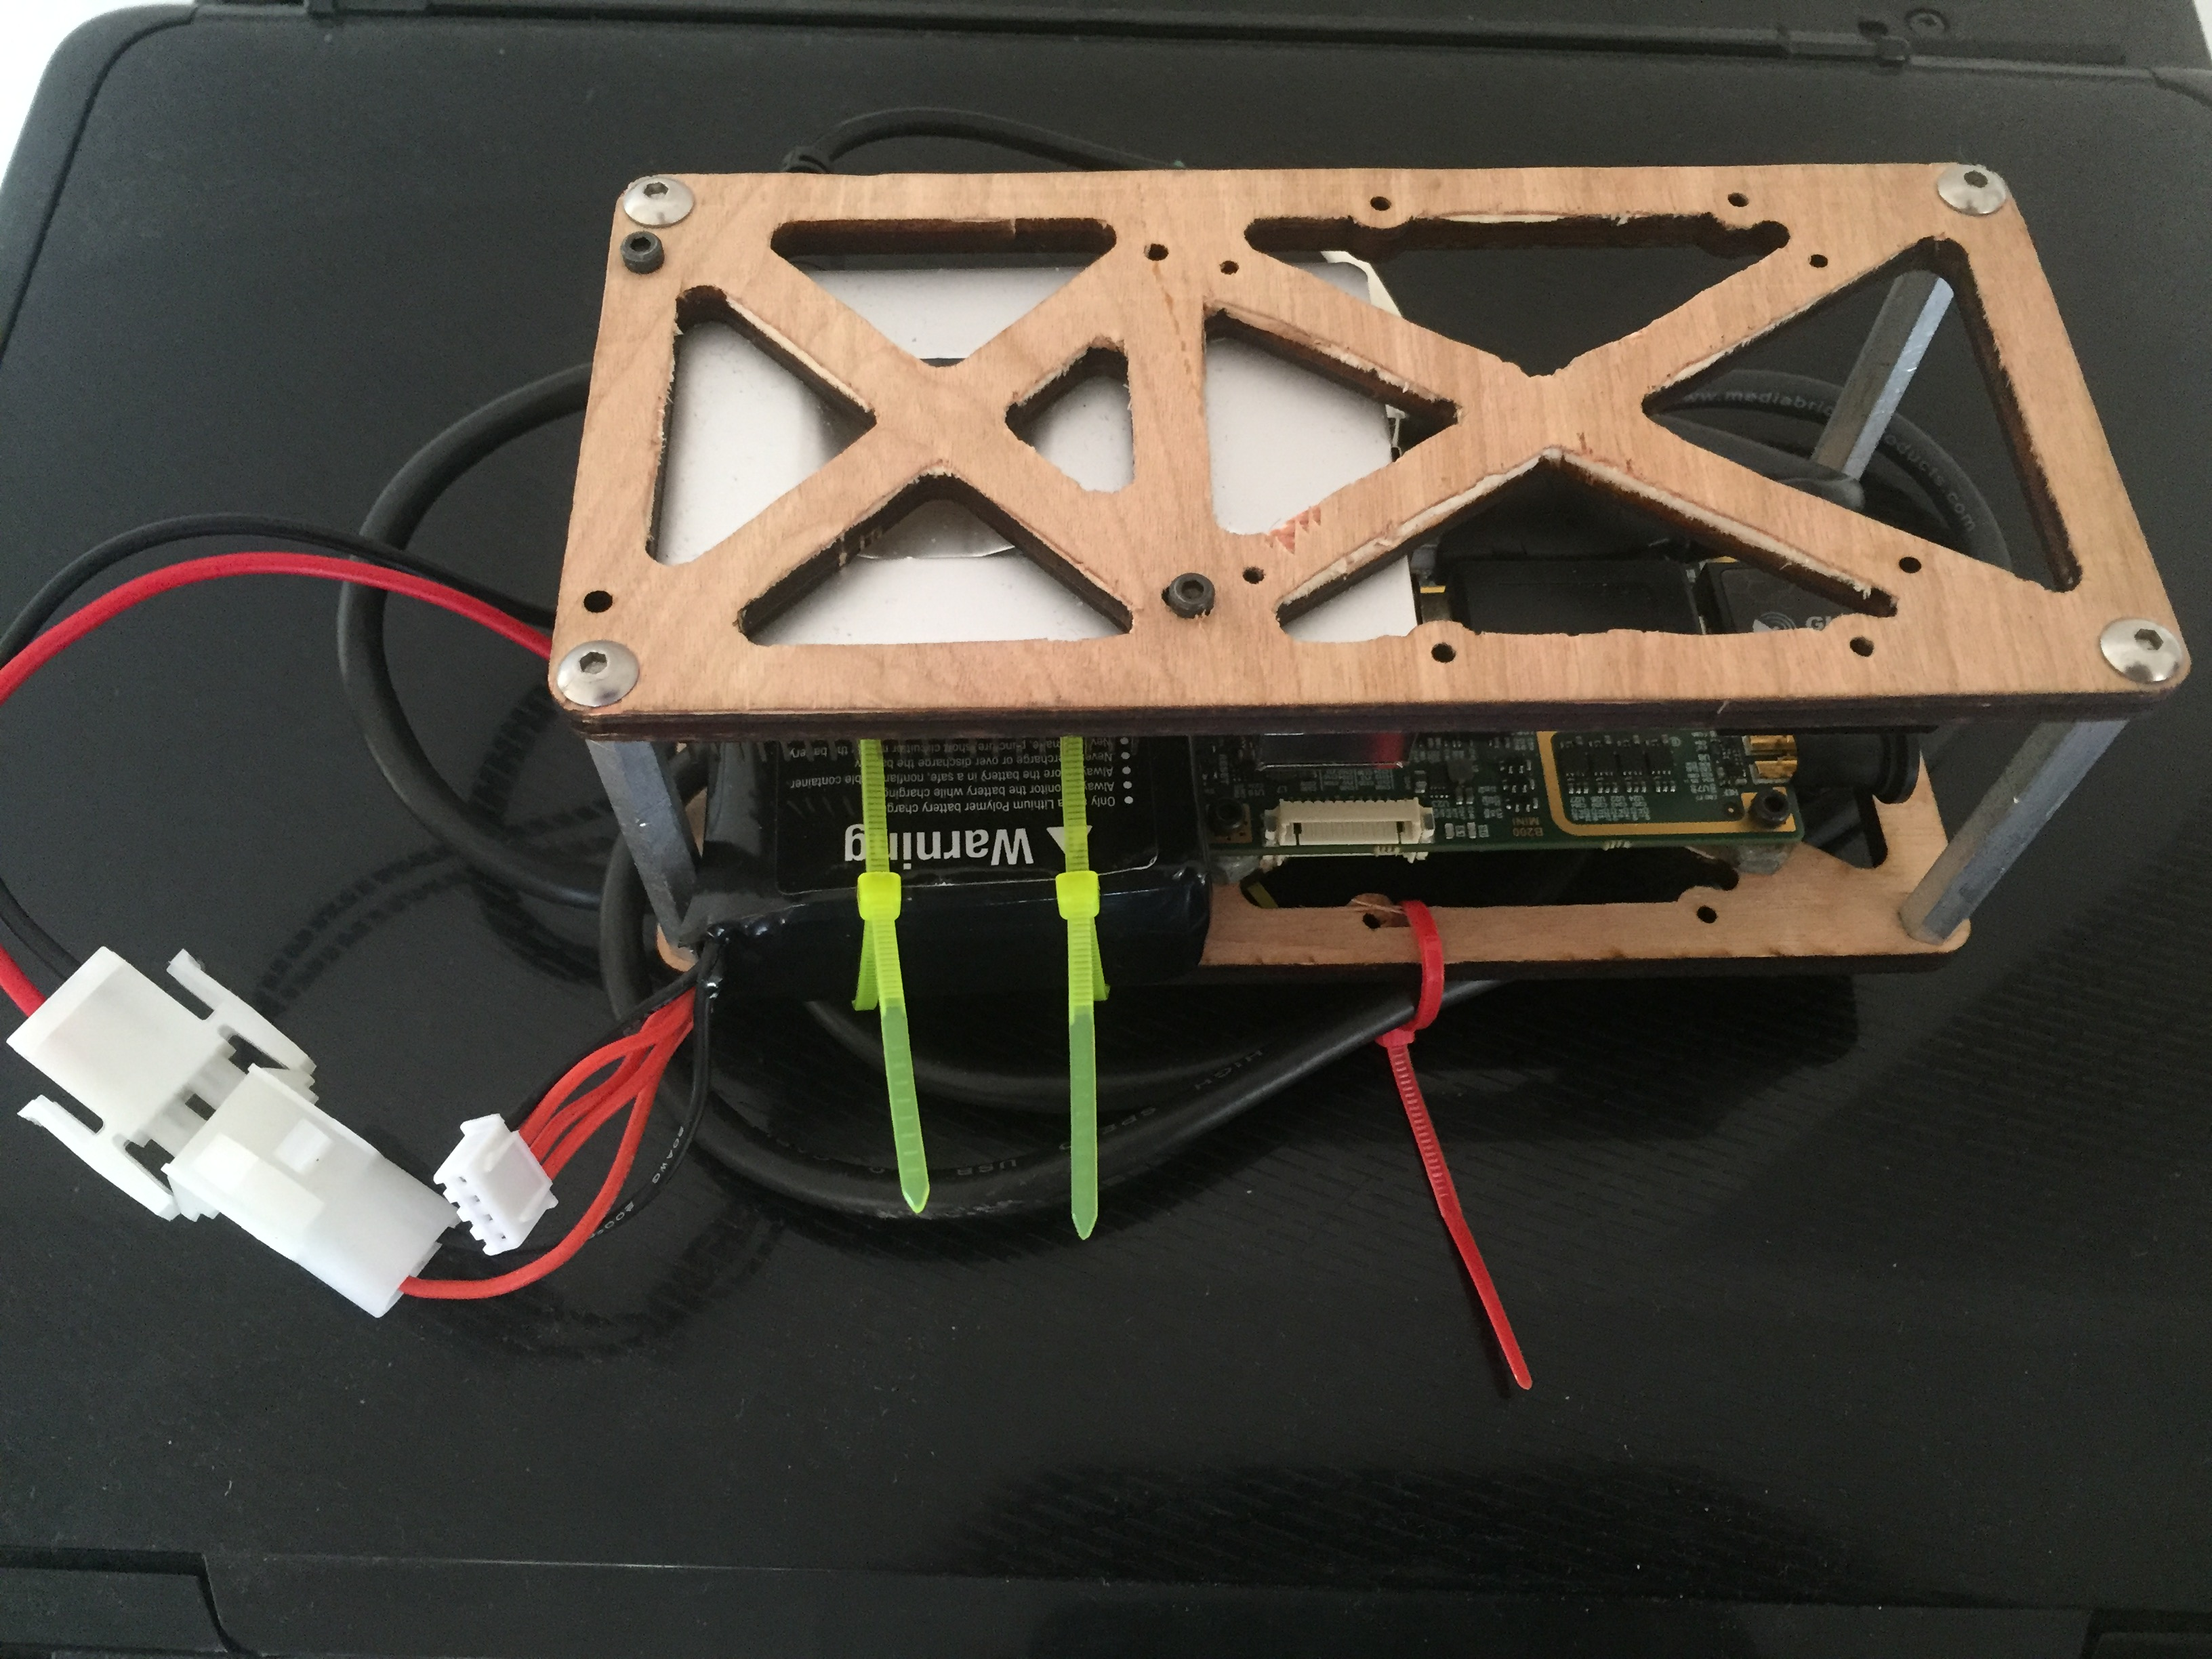
\includegraphics[width=0.70\textwidth]{img/Overhead_of_box.JPG}
	\caption{Overhead view of the encasing of the MASDR system}
	\label{fig:overhead_of_box}
\end{figure}\par
The two wooden panels were created identically to reduce design time and fabrication time. Screw holes were precut into the wood to ensure mounting the components wouldn't split the wood. This enclosure was mounted to the bottom of the drone using the hardware mount on the drone detailed in Section \ref{Mounting}. \par

To power the system, an 11V LiPo battery was used in combination with a 5V transformer to step down the voltage for use by the UP Board. The battery and converter were connected using connectors seen in Figure \ref{fig:connectors}, so that the battery could be disconnected when not in use. To prevent any mishandling of plugging the battery in backwards, a male molex connector was soldered to the transformer and a female molex connector was soldered to the battery.
\begin{figure}[ht!]
	\centering
	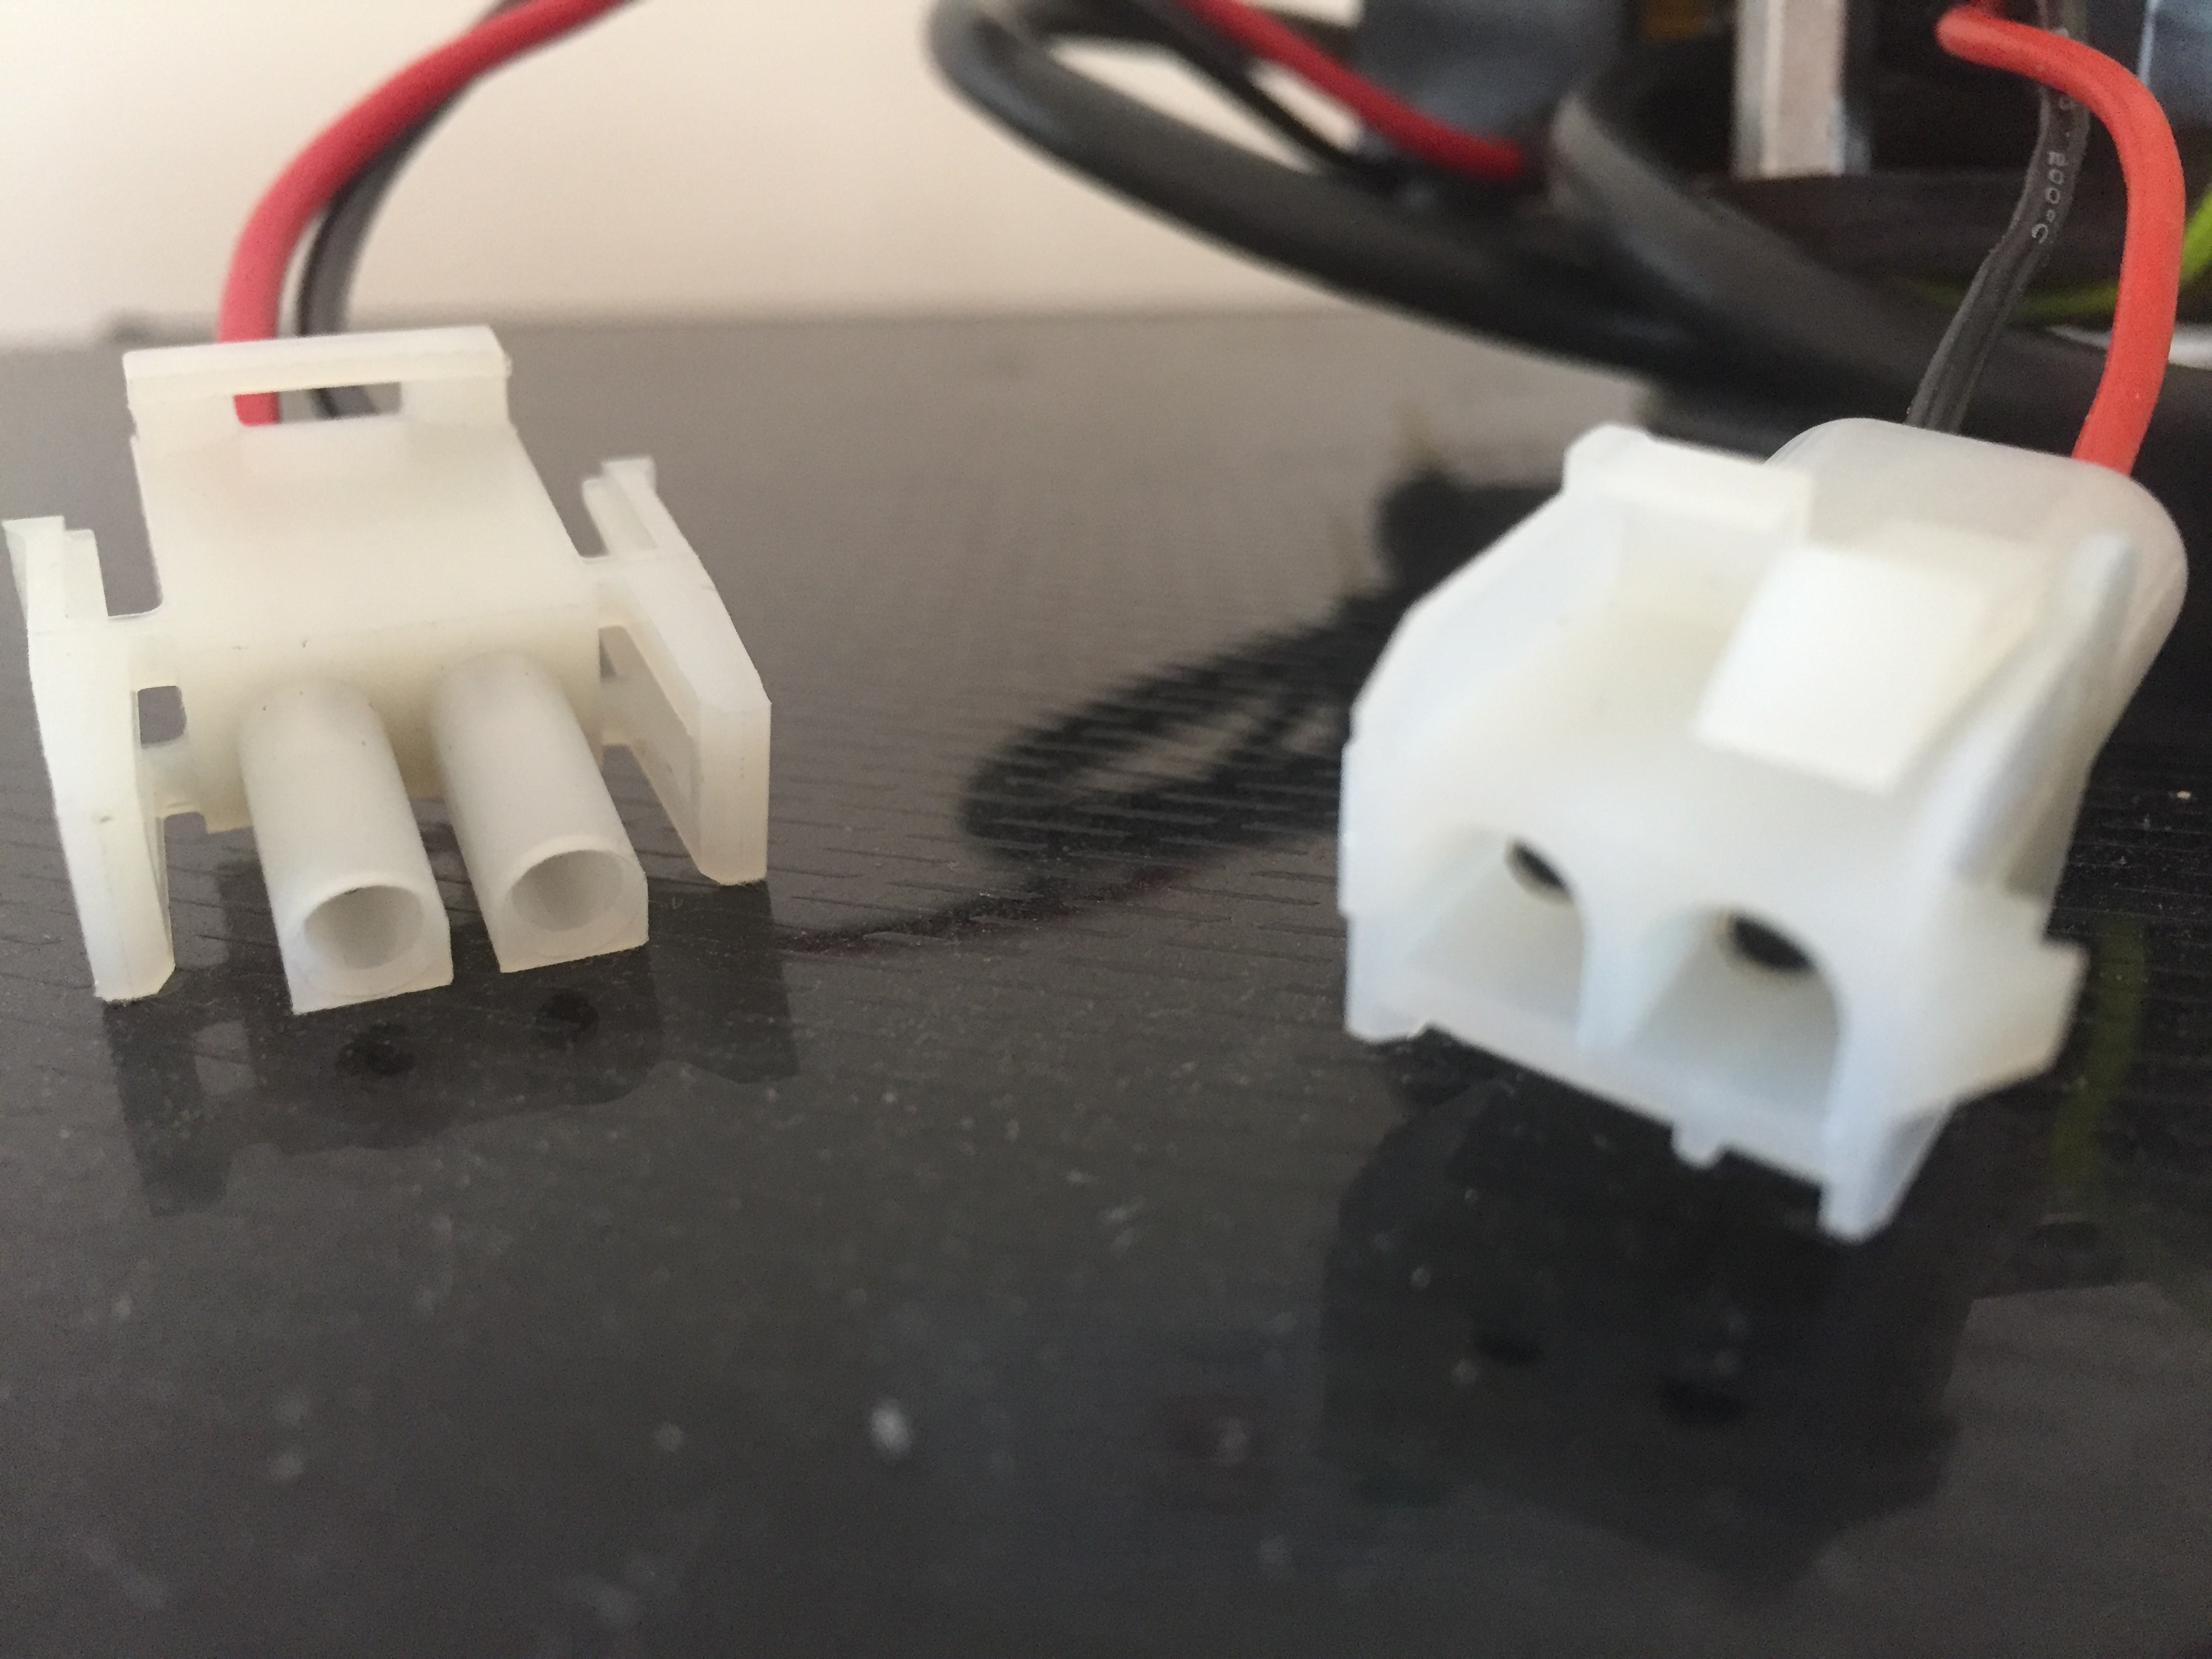
\includegraphics[width=0.70\textwidth]{img/connectors.JPG}
	\caption{Connectors for the battery. The male molex connector (left) is connected to the transformer and the female molex connector (right) is connected to the LiPo battery.}
	\label{fig:connectors}
\end{figure}\par
There were two transformers that were purchased, the Nextrox converter was the one that directly converted 12V down to 5V at 3A, and the DROK converter was the other which was an adjustable knob that ranged from 8V-35V to 1.5V-24V at 5A. Unfortunately the first transformer worked for the first few trials and the second just outright did not work out of the box. The first transformer that was used in the system failed because it became disconnected from the UP Board when power was applied. This transformer was a buck converter which can fail when an output isn't connected due of the failure of a MOSFET or diode\textbf{Add citation for here eventually}. The second transformer's adjustable knob did not change the ratio at which the voltage was being output despite multiple attempts and methods. A new transformer was purchased to replace the malfunctioning transformers. \par

The UP Board is connected to the 5V transformer using a barrel jack. The male connector was soldered onto the output of the transformer. The UP Board is the main system with everything else connected to it through USB or I2C. It was mounted upside down on the top panel as shown in Figure \ref{fig:box_usb_view}.
\begin{figure}[ht!]
	\centering
	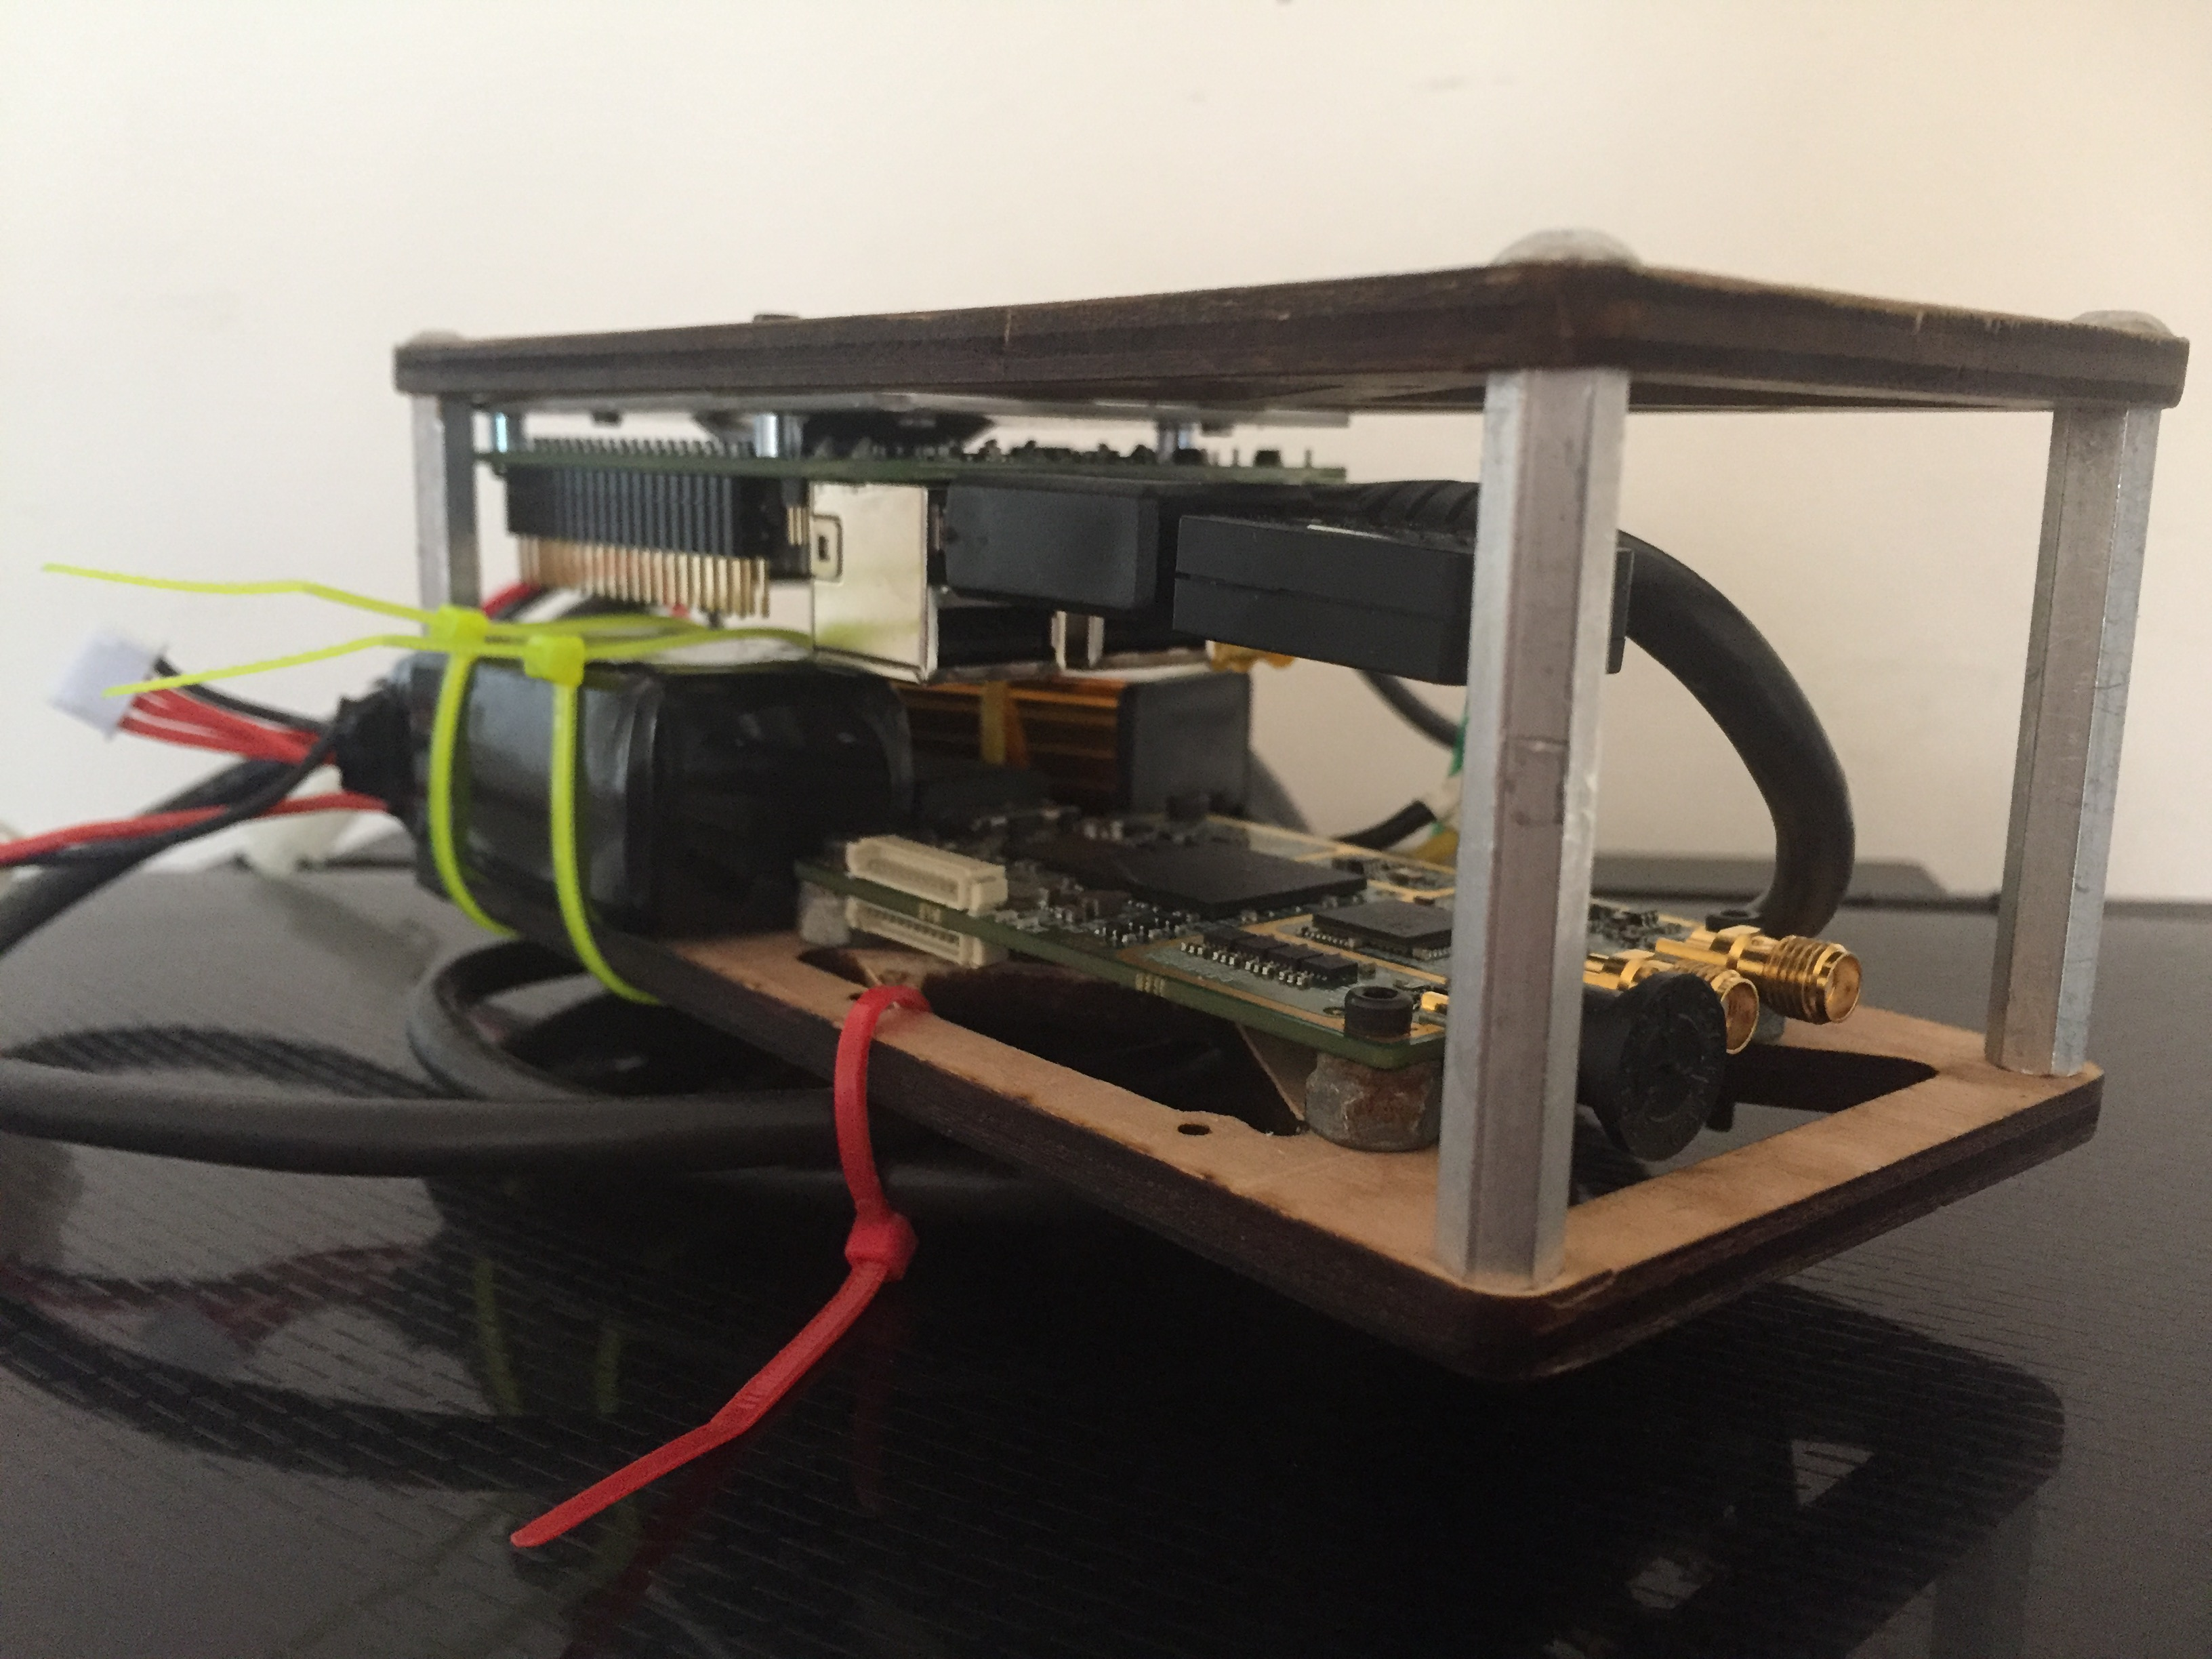
\includegraphics[width=0.70\textwidth]{img/box_usb_view.JPG}
	\caption{Angled side view of the encasing with the UP Board connected to the top panel with the GPS and USB cable to the B200-Mini. The golden transformer and the battery are positioned directly under the UP Board on the bottom panel. The B200-Mini is connected to the bottom panel and is the closes board to the camera.}
	\label{fig:box_usb_view}
\end{figure}\par
The GPS is connected to the UP Board using an micro USB to USB adapter. Integration and operation of the GPS proved to be a challenge. The GPSD library that was used to interface with the GPS had permission issues that caused the GPS data to not be read by a C++ program. After the permissions were set correctly, the MASDR program was able to correctly read the GPS data.\par

The magnetometer was to be connected to the UP Board using the I2C pins. Communication between the UP Board and the magnetometer was never established after multiple attempts. The UP Board would send a signal to the magnetometer, but never received a response. This could be due to a lack of a Linux driver or a faulty board. A Linux driver for the magnetometer wasn't provided by the manufacturer and the time line of the project made it unfeasible to write a driver by hand.\par

The B-200 mini was attached to the bottom panel of the casing. It communicated to the UP Board through a wired USB connection. The 900MHz and 2.4GHz antennas were connected to the SMA connectors on the mini. The 2.4GHz antenna required an adapter because the connector on the board was not compatible with the one on the antenna. During testing, it was realized that the transmission from the board was not working. Upon further inspection it was noticed that a component had broken off the board. Another board was borrowed from a lab to verify that the original board was faulty. The transmission test ran successfully on the board from the lab. A working board and the broken board are shown in the Figure \ref{fig:working_mini} and Figure \ref{fig:broken_mini} respectively.
\begin{figure}[ht!]
\begin{minipage}{.5\textwidth}
  \centering
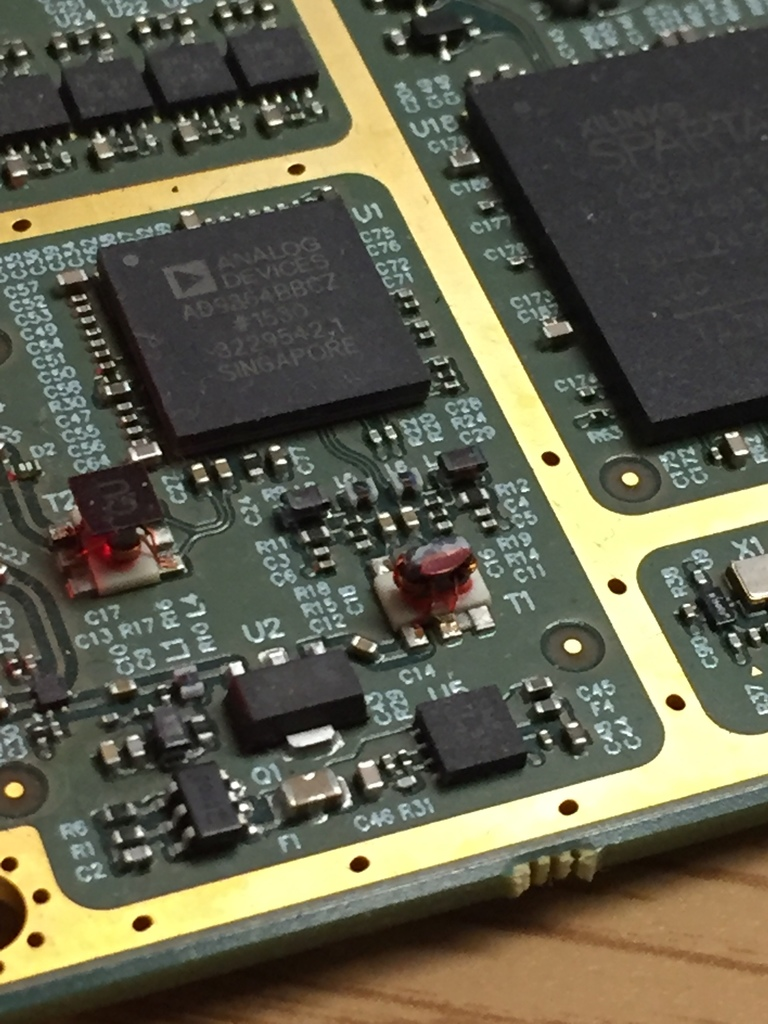
\includegraphics[width=0.9\textwidth]{img/working_mini.jpg}
\caption{The functional B200-mini}
\label{fig:working_mini}
\end{minipage}
\begin{minipage}{0.5\textwidth}
\centering
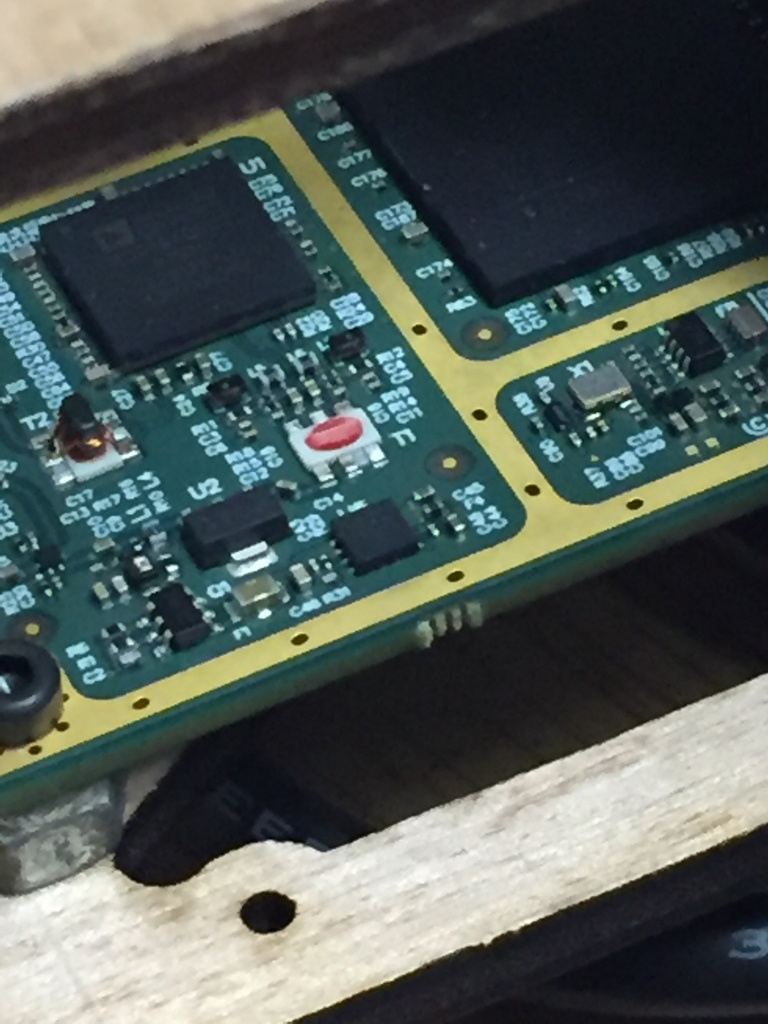
\includegraphics[width=0.9\textwidth]{img/broken_mini.jpg}
\caption{The nonfunctional B200-mini}
\label{fig:broken_mini}
\end{minipage}
\end{figure}

This component may have broken off during transport to and from meetings or because of vibrations during in flight testing. \par

The complete system mounted on the drone is shown in Figure \ref{fig:drone_and_box}.
\begin{figure}[ht!]
	\centering
	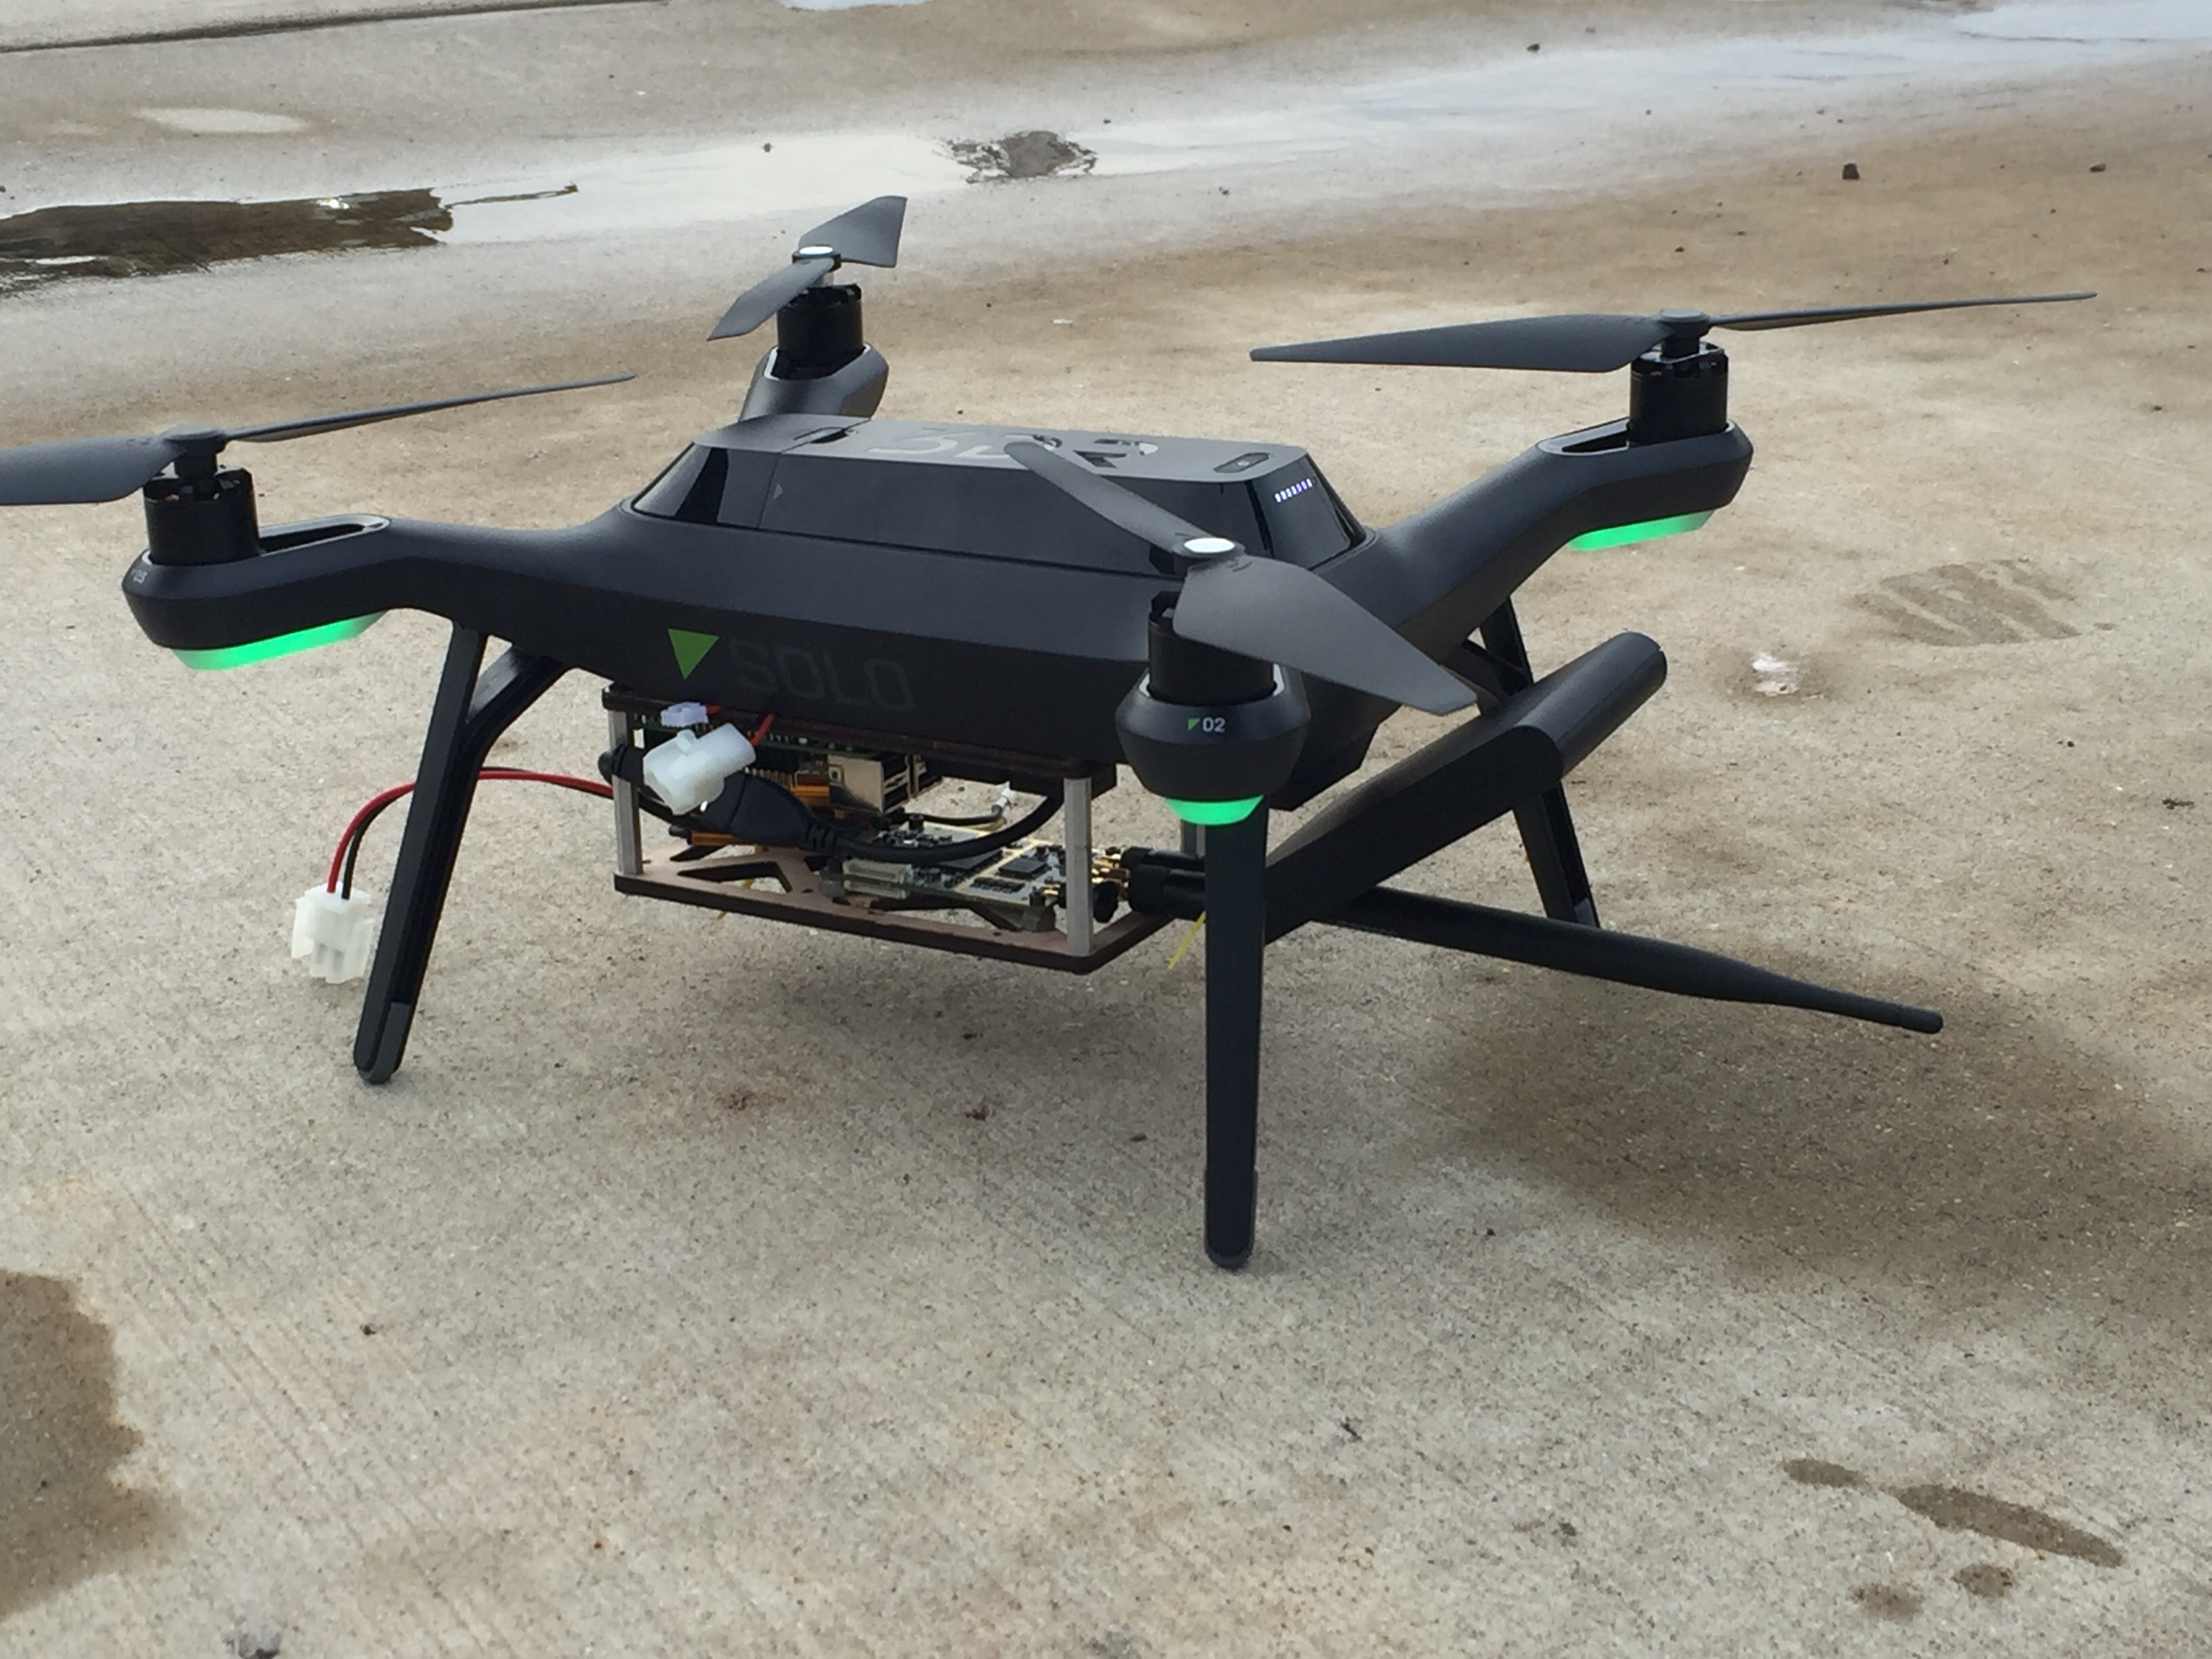
\includegraphics[width=0.70\textwidth]{img/drone_and_box.jpg}
	\caption{The complete system mounted on the drone. In flight testing was done with this setup.}
	\label{fig:drone_and_box}
\end{figure}
\par

% \section{Code Framework}
% What kind of results are even here? How the framework works I think
% If you don't do that you should do the other thing.
\section{Drone Control}
To reduce interference when sensing signals, the WiFi cards on the controller and drone had to be replaced because the communication frequency and the sensing frequency were the same value. In order to replace these WiFi cards, research had to be done to determine which driver was used on the drone. This ended up being the ath9k driver, which was compatible with a wide range of Atheros based cards. Despite the guarantee of compatibility, the first purchase of the R11e-5HnD MikroTik MiniPCI-E wireless card ended up unused, due to the large heat sink that could not fit conveniently into both the controller and drone. Furthermore, the connectors would also require adapters to connect to the antennas. This led to the second purchase of the SparkLAN WPEA-121N MiniPCI-E Half-Size wireless card, which required a bracket to be mounted. The replacement of the WiFi cards in the controller was done first, because the controller acts as a WiFi base station. This makes it easier to test 5 GHz functionality. The replacement went smoothly. However, the controller was still communicating at 2.4GHz. Upon checking the software, it detected that the WiFi card installed was capable of communicating at 5GHz. Therefore, the controller's networking scheme was modified such that it would persistently communicate at a specific channel (5GHz). After these changes, there was trouble SSHing into the controller. One possible explanation is that the antennas are incapable of transmitting at 5GHz. Limited with time and the scope of the project, it was not possible to obtain antennas to replace on the controller and drone. Due to this reason, the drone's WiFi card was not replaced, and both the controller and drone were factory reset to operate at 2.4GHz. \par

A python script was written to briefly take control of the drone and rotate while holding a constant position and altitude. The script used the Dronekit API provided by 3DR. The script was packed up with all necessary libraries and sent to the drone awaiting execution. When the command is given by a computer connected to the controller's WiFi network, the script runs, taking over control of the drone and rotating it. The API did not provide a way to set a constant rate of rotation, so instead a nonblocking call to rotate a certain amount was used in conjunction with timed sleeps to achieve a continuous rotation of 360 degrees. Attempts to map the script to a button on the controller were unsuccessful. The 3DR developers guide notes a future API called \"Smart Shots\" that allows commands to be mapped to buttons on the controller, but it was not available at the time of this project.

\section{Spectrum Sensing}

In order to monitor the signal strength of our received data, the RSSI localization technique was used. RSSI was measured by taking the average signal power across a 20 MHz 802.11 wifi channel. This RSSI measurement was taken by using the USRP B200 Mini’s get\_rx\_sensor command.  This command returns the corresponding RSSI value as a double in dBm format.  However, since a WiFi transmitter is not transmitting all of the time, there are sharp changes in RSSI measurements since the USRP is receiving both when there is a signal and when there is none.

\begin{figure}[h]
	\centering
	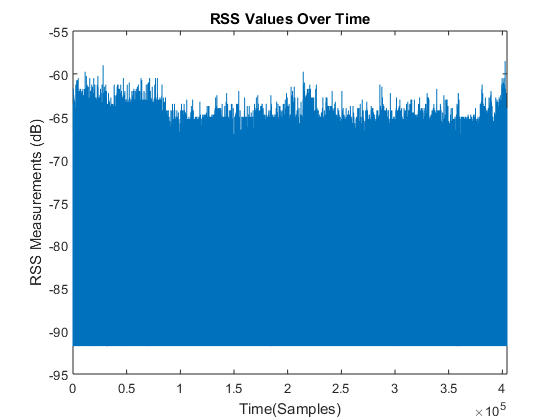
\includegraphics[width=0.70\textwidth]{img/rss_vals_test.png}
	\caption{This graph shows how the RSSI of our received signal can dramatically change.  These sharp transitions in RSSI values are due to the transmitter not always continually transmitting.}
	\label{fig:rss_values}
\end{figure}
In order to have an accurate RSSI, RSSI reports that are under the noise floor must be filtered out. A detection threshold of -85 dBm which was selected, as it is above the noise floor.  The output for our RSSI measurements only record noticeable signals.  

Corresponding RSSI values were used to estimate the distance of the transmission that was sensed.  The localization algorithm depended upon this calculation in order to accurately locate a signal source. the distance equation used was:

 \begin{align}
\label{eq:rss} RSSI &= 10\alpha log(d) \\ 
d &= 10^{(RSSI-RSSI_{calibration})(-10\alpha)} + d_{calibration} \label{eq:rss_dist}
\end{align}\\
These equations were mentioned previously in Section \ref{back:radio_loc}
Based on some field testing, this equation has been fairly accurate.\par

\begin{table}[ht]
\centering
\label{table:RSSI_Results}
\begin{tabular}{|l|l|l|} \hline
  RSSI (dBm) & Observed Distance (Meters) & Theoretical Distance (Meters) \\ \hline
  -50 & 3 & 3.2 \\
  -60 & 9 & 10 \\
  -70 & 26 & 31.62 \\ \hline
\end{tabular}
\caption{As you can see by our observed RSSI values, our RSSI to distance calculation allows us to reasonably relate received signal strength to how far away a transmitter is located.}
\end{table}\par

When the drone was tested, received signal strengths were between -65 to -80 dBm which falls within the expected power range of desired signals, as the sensing platform was 100 ft or 30 meters away from the transmitter. 

%IQ_TO_FILE
In addition to calculating RSS values, a C++ program separate from the code framework
was written. This program, called iq\_to\_file, was created as a foundation with 
which to work with. It became the testbed for specific elements of MASDR, since it
was already capable of logging. The code for this section is in Appendix \ref{app:iq_to_file}. 
This program is built on the rx\_samples\_to\_file example that Ettus Research provides 
with the UHD. This program already had the desired base functionality, so it proved
to be a good starting point. The program was then stripped of unnecessary functionality,
including the command-line interface. \par
With the extraneous functionality removed, components of the MASDR framework were
added, in order to test them separately. The matched filter, RSS measurements, 
and GPS modules were the sections added. This allowed for post-process localization. In order to 
save these values properly, they were packed into the complex type that was being
used to save IQ samples. In order to make it possible to pull these values out
in post-processing, they were given an unrealistic imaginary value. with each different 
module getting a different imaginary value. The matched filter outputs got 
a flag of 1000. GPS X, Y and Z coordinates were given flags of 2000, 3000, and 4000,
respectively. RSS values got a flag of 5000. These values were written with each 
buffer of samples received. This makes it easier to align results when processing.\par
%MATLAB
Once a data file was recorded, it was processed using a MATLAB script. This script 
is in Appendix \ref{app:matlab_proc}. This script reads in the .dat file produced 
by iq\_to\_file, as floats. It then separates the data into in-phase and quadrature
components. Then, after pre-allocating buffers, the script pulls out the non-IQ 
samples. The matched filter values and the RSS measurements are then plotted. The
script used to plot the received signal, but with longer record times, this
becomes impractical or impossible.

\section{Spectrum Localization}
%GPS
The GPS was to be used to gather location data to allow for post processing. Unfortunately the GPS was non-functional during the test due to it being unable to locate satellites during the tests. Therefore, in order to use the data gathered in the test conducted on December 11, 2016, GPS 
data was pulled from the drone. This was done using a command-line interface that 
3DR provided online \cite{3dr_devguide}. Unlike the other logs that were pulled using this method,
the GPS information was logged in a Dataflash log. This format saves the information
in MAVlink packets, making it easier to transmit to a base station but harder
to post-process. To deal with this, the Ardupilot Mission Planner software was 
installed \ref{ard_mplanner}. This software is capable of taking the dataflash logs
generated by the 3DR Solo and converting them into a format that's easier to
process. Using this software, the logs for the flight on December 11, 2016 were 
converted to MATLAB data files. The relevant GPS information was then pulled from
the larger data set. \par
%Probably put script here

%KF Simulation
Because of the complications with the GPS measurements, the 4-state Kalman filter
was modeled in MATLAB. The script can be found in \ref{app:kf_sim}. The script 
initializes the matrices as described in section \ref{methods:kf}. A noisy input
with a constant x velocity 1 and y velocity 1 is initialized. Arbitrary variance
values are used in $\matr{P}$ and for the noise covariance matrices $\matr{Q}$
and $\matr{R}$. Plots of the resulting predictions are shown below. 
\begin{figure}[ht!]
\begin{minipage}{.5\textwidth}
  \centering
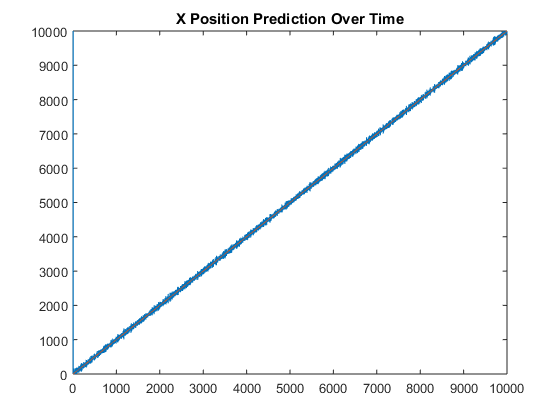
\includegraphics[scale=0.5]{img/kf_xpos.png}
\caption{X position predictions from Kalman filter simulation.}
\label{fig:kf_xpos}
\end{minipage}
\begin{minipage}{0.5\textwidth}
\centering
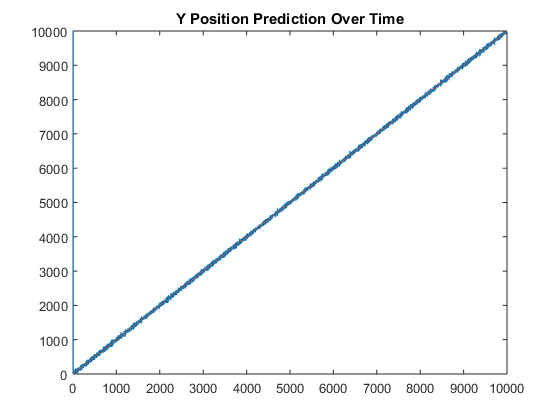
\includegraphics[scale=0.5]{img/kf_ypos.png}
\caption{Y position predictions from Kalman filter simulation.}
\label{fig:kf_ypos}
\end{minipage}
\end{figure}
\begin{figure}[ht!]
\begin{minipage}{.5\textwidth}
  \centering
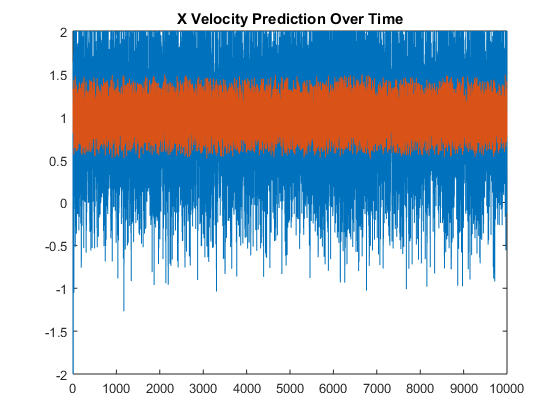
\includegraphics[scale=0.5]{img/kf_xvel.png}
\caption{X velocity predictions from Kalman filter simulation.}
\label{fig:kf_xpos}
\end{minipage}
\begin{minipage}{0.5\textwidth}
\centering
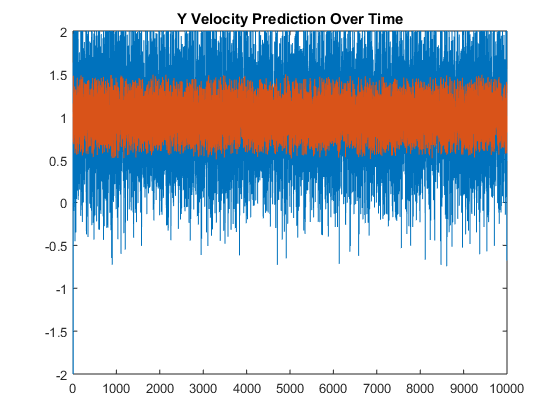
\includegraphics[scale=0.5]{img/kf_yvel.png}
\caption{Y velocity predictions from Kalman filter simulation.}
\label{fig:kf_ypos}
\end{minipage}
\end{figure}\par
As seen above, the resulting predictions that come from the Kalman Filter are
decent, but not too much of an improvement. This is due to a number of factors.
The first factor is the fact that there are no direct measurements of velocity.
Because of this, the resulting velocity measurements already introduce some error.
Another factor is the choosing of the various parameters. This was done in a fairly
arbitrary manner, due to time constraints.
\subsection{Mapping Script}
The script used to display the measured signal strengths was designed for post-proccesing use, taking in a text file of locations and their corresponding RSS values. The processing portion of the script is written in python, and can be found in Appendix \ref{app:map_script}. Equation \ref{eq:rss_dist} is used to calculate the raw distance to the signal. The Pythagorean Theorem is then used to eliminate the altitude component of the distance as can be seen in Figure \ref{fig:dist_pyth}. The latitude, longitude, and land-based distance are then formatted into a template string for each point at which a signal was detected.\par
\begin{figure}[ht]
\centering
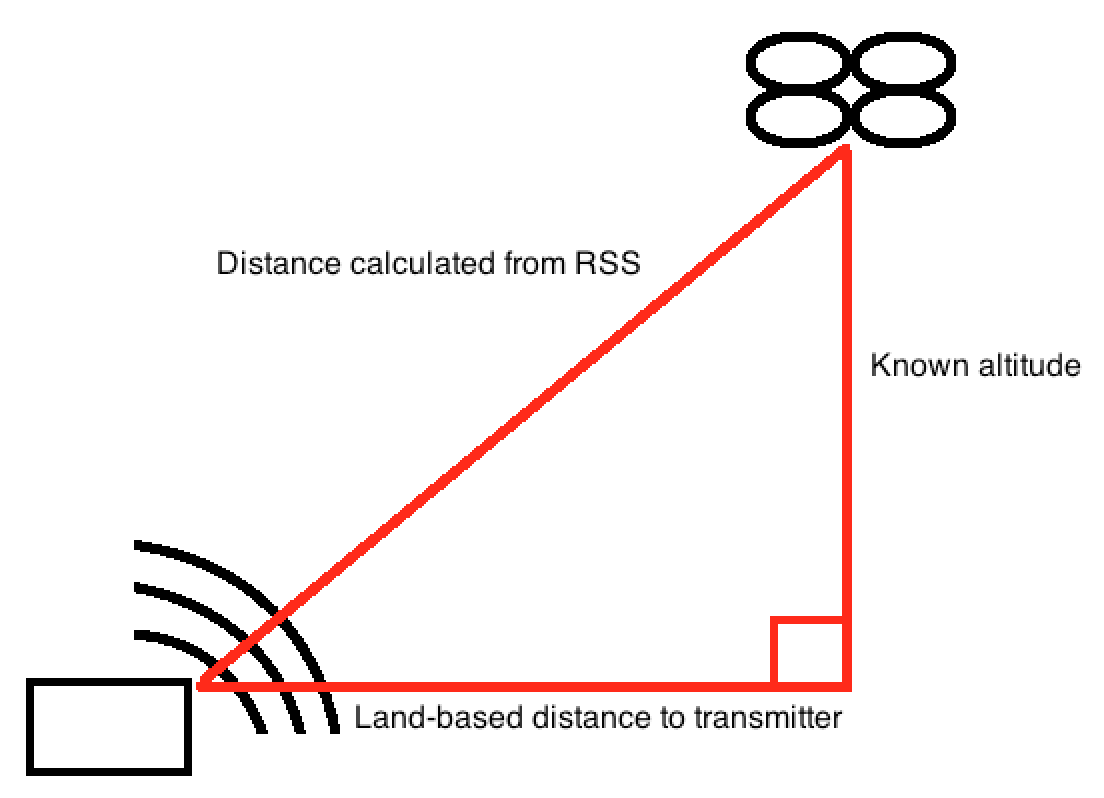
\includegraphics[width=0.70\textwidth]{img/distance_pythag_diagram.png}
\caption{Diagram showing right triangle used to calculate land-based distance from the calculated distance and a known altitude.}
\label{fig:dist_pyth}
\end{figure}
The formatted strings are inserted into a template html file, primarily composed of a javascript block that calls into the Google Maps API. Using the drawing tools in the API, rings are drawn on the map corresponding to the calculated distance. An example output screenshot of a generated map has been included in Figure \ref{fig:map_localize}. The actual output is a webpage with a Google Maps instance running in it, so the map is fully interactive, with the ability to zoom in and scroll around as well.
\begin{figure}[ht]
\centering
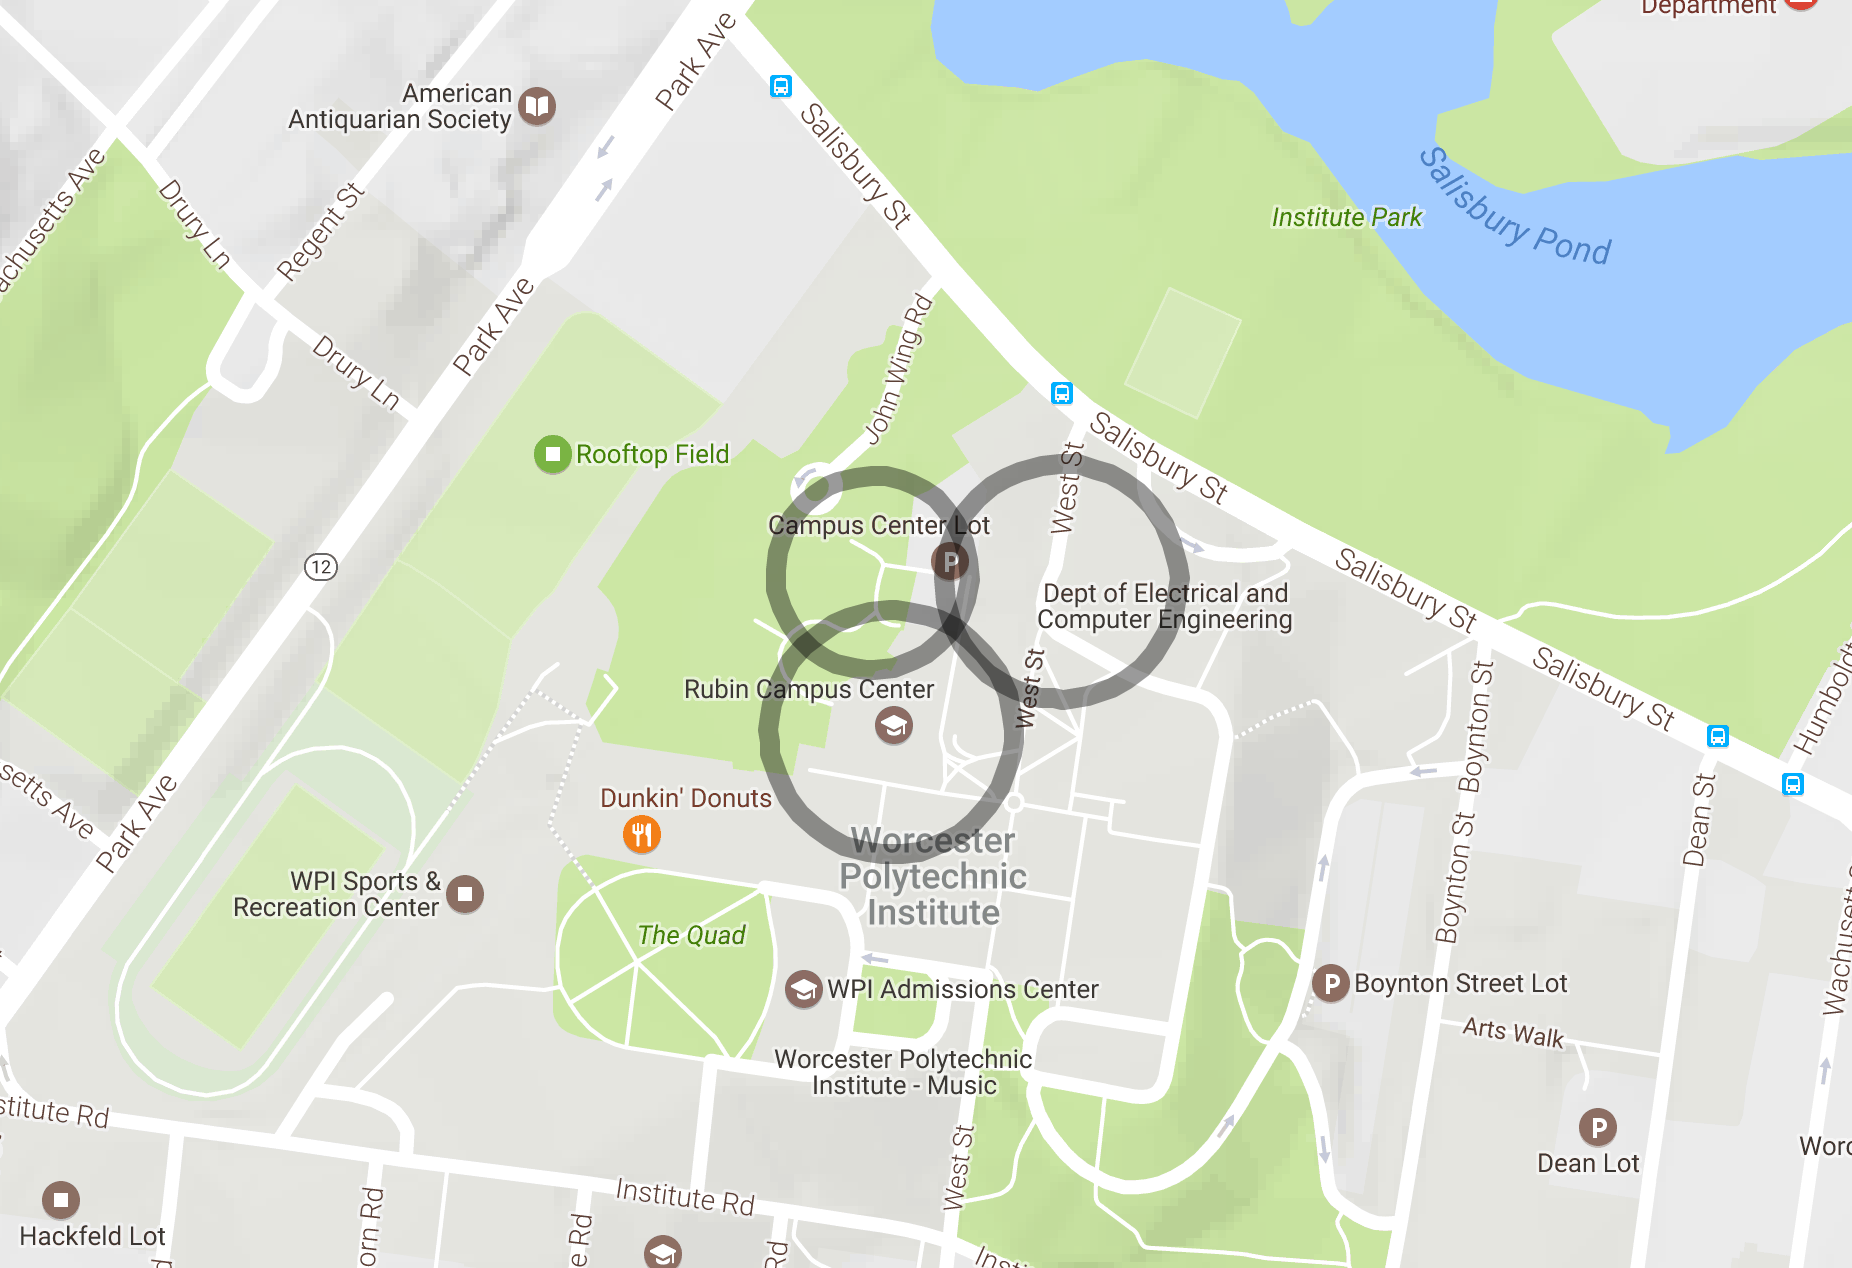
\includegraphics[width=0.70\textwidth]{img/localization_map_visualization.png}
\caption{Map-based localization example. The rings drawn are calculated from RSS values based on samples taken at the centers of each ring.}
\label{fig:map_localize}
\end{figure}

\section{Transmit To Ground}

In order to reduce the amount of processing done onboard the drone, a ground receiver was created.  This ground receiver receives important information such as the location, power level, and frequency in which a signal was detected at.  This information is transmitted from the MASDR platform to a ground-based RTL-SDR.  

Differential binary phase shift keying or DBPSK modulation was used as the communication protocol for transmission to the ground receiver. This ensures a reduced bit error rate. A DBPSK receiver and transmitter was implemented using GNURadio. The receiver side of the system used the flowgraph shown below:

\begin{figure}[h]
  \centering
  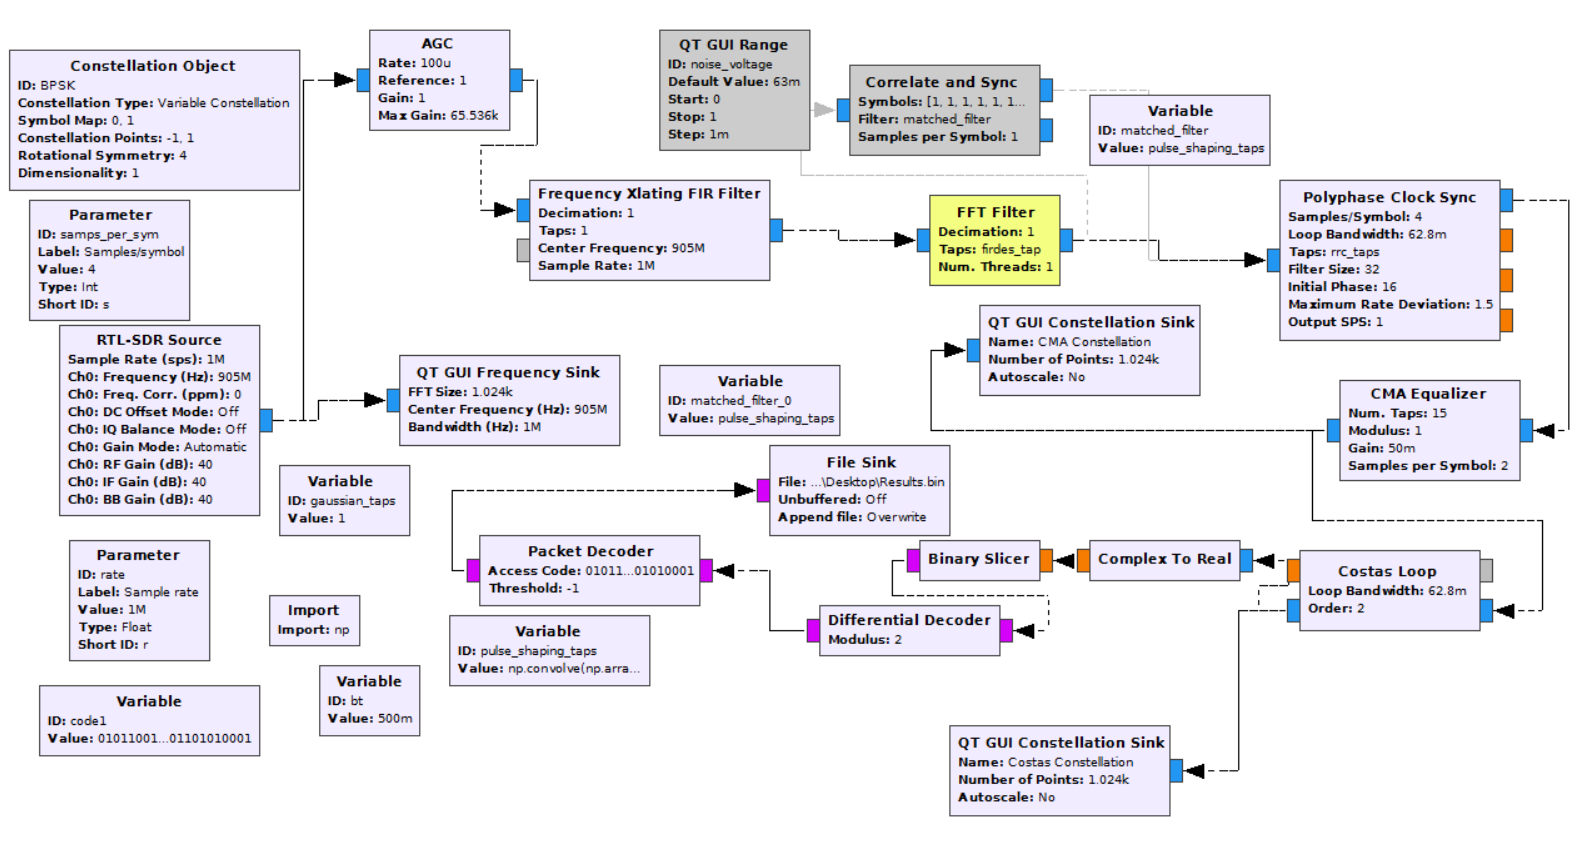
\includegraphics[width=0.70\textwidth]{img/rxflow.PNG}
  \caption{This flowgraph was created in GNU Radio to receive and demodulate the received DBPSK waveform. This is done by using the QT GUI development environment in GNU Radio}
  \label{fig:rxflow}
\end{figure}

This program receives a binary file source which is an array of the data to be sent. This passes through a packet encoder, which encapsulates all of the data from the binary file into a packet with a preamble and an access code.  This is ensures that the receiver will sync correctly to decode the transmitted data.  Then after this, it goes through a constellation modulator that modulates the binary information into a corresponding analog waveform. It is then transmitted using the USRP with at central frequency of 905 MHz.  Before using the receiver, a spectrum monitoring tool for the RTL-SDR called SDR\# is used to confirm that the USRP is transmitting on this frequency.

\begin{figure}[h]
  \centering
  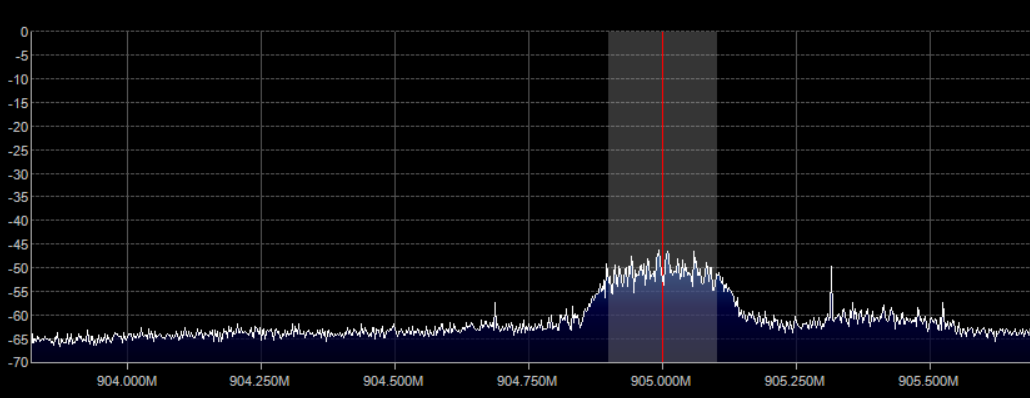
\includegraphics[width=0.70\textwidth]{img/rxspectrum.PNG}
  \caption{This photo shows an FFT with a center frequency of 905 MHz which is what frequency our USRP is transmitting at.  This waveform was created by using SDR\# on an RTL-SDR.}
  \label{fig:rxspectrum}
\end{figure}

This signal is then received by the RTL-SDR.  However, significant handling of the signal must be taken care of before the correct information can be demodulated. After this a Frequency Translating FIR Filter was used as a bandpass filter, removing extra signals that might be around that band. After this, a series of three more functions were used. First, a polyphase clock sync is used to perform timing synchronization with the transmitter. This is done by using two filter banks that use a matched filter on a signal’s pulse shape. A root raised cosine filter for our pulse shape since our transmitter is using a root raised cosine filter. This synchronized signal is then sent through a CMA Equalizer which equalizes modulated baseband signals. Then, a Costas Loop is used in order to provide adequate phase correction so that the received signal's constellation is locked in phase for the entirety of the transmission.  Our results after all of this signal processing are as expected with the received BPSK signal. 

\begin{figure}[h]
  \centering
  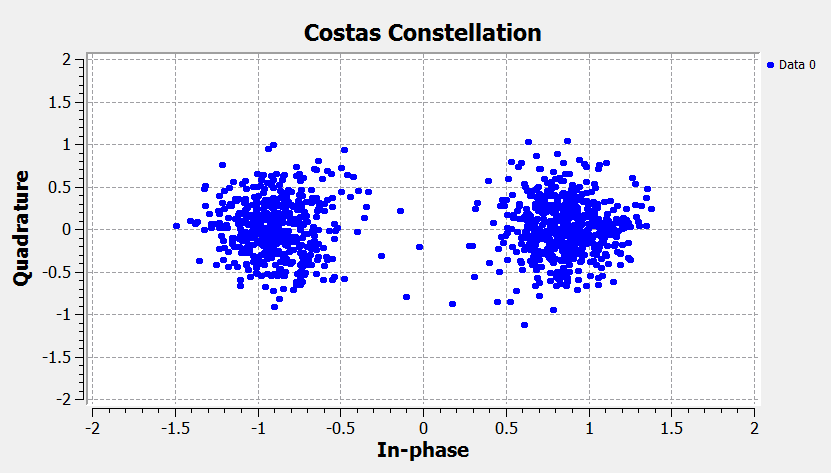
\includegraphics[width=0.70\textwidth]{img/constellation.PNG}
  \caption{This is a photo of our received constellation when we are finished performing the timing offset and phase correction on the transmitted signal.  This constellation is taken when the signal strength was at -55 dBm which is the expected signal strength when the drone is receiving signals in the air.}
  \label{fig:constellation}
\end{figure}

This constellation is then sent through a differential decoder and a packet decoder, to extract the payload out of the packetized binary information. This data is then uploaded to results file on the ground receiver’s main computer.

\section{Platform Deployment}
The platform on the 3DR Solo was tested in the two most applicable scenarios, the rural environment and the urban environment. The tests were conducted in secluded areas to prioritize privacy and safety concerns. The tests consisted of mounting the platform onto the 3DR Solo, flying the drone in a procedural flight path as seen in Figure\ref{fig:test_setup} to collect IQ data, and processing the data for the mapping and the localization of signals around that area. The signals in our case, would be the controller access point. 

\begin{figure}[ht!]
	\centering
	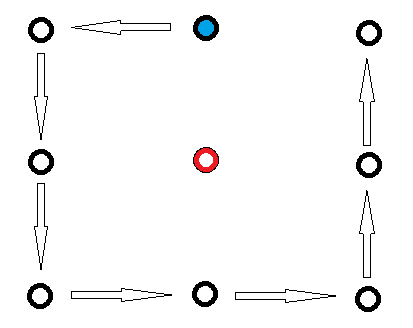
\includegraphics[width=0.70\textwidth]{img/Test_Plan.png}
	\caption{3x3 diagram of test flight plan. The red circle represents where the controller was placed, and the blue circle represents where the drone was started.}
	\label{fig:test_setup}
\end{figure} \par

The simulation of the rural environment was organized at Professor Wyglinski's property on December 11th, 2016. In order to get the least interfering wifi signals, he turned off his WiFi, and he authorized the flight of the drone on his property. The testing environment consisted of high rise trees that surrounded the area and grew up to an average of 80ft. The resulting mapping and localization of the area is provided in \ref{rural_test}.

\begin{figure}[ht!]
	\centering
	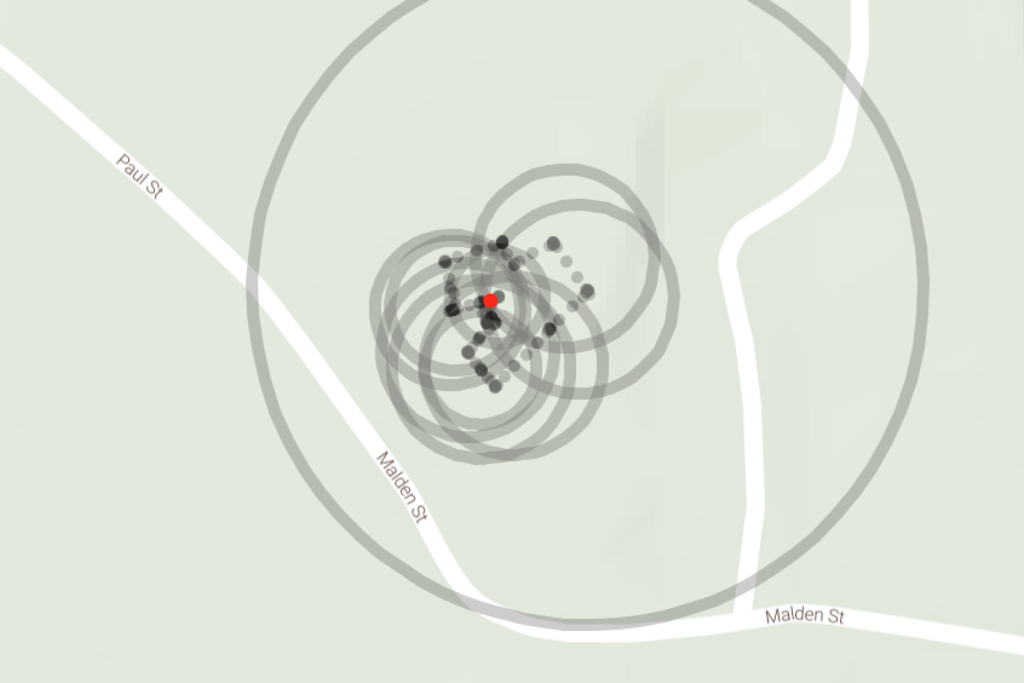
\includegraphics[width=0.70\textwidth]{img/ruraltest.png}
	\caption{The result of the test flight in a rural environment. The red dot shows where the actual access point was located. The black dots represent the GPS locations of where the drone traveled, and the their shades illustrate the length of time the drone was at that location. The black hollow circle depicts the localization of where the drone thinks the access point may be based on GPS and RSSI measurements. The larger hollow circle represents a measurement close to the noise floor.}
	\label{fig:rural_test}
\end{figure} \par
The simulation of the urban environment was organized at the Gateway Park garage on campus, on December 16th, 2016, after having gotten permission for the test from campus police. This WiFi of this area was uncontrolled, with various public and private access points active. This better simulated an urban environment. There were not many tall buildings around, limiting the applicability of the test on denser urban areas. 


\section{Summary}
In this section, the results achieved in this MQP were discussed. This focused primarily on the design and implementation of the system, as well as the processing of the data collected. Overall, the team was able to create a good foundation on which aerial sensing methods can be applied.
